\section{Verteilte Anwendungen mit RMI}

Wenn man eine verteilte Java-Anwendung entwickeln soll, bei der Kommunikationsprotokoll und Client- und Server-Seite in Java implementiert werden, ist \textbf{RMI} die bessere Alternative gegenüber  \textbf{Sockets} (vgl.~\cite[311]{Oec22}).\\


\begin{tcolorbox}
    \textbf{Remote Method Invocation} ermöglicht das Aufrufen von Methoden auf Objekten, die sich auf demselben oder einem anderem Rechner als der Aufrufer befinden, und damit als unterschiedliche Prozesse in unterschiedlichen Adressräumen ausgeführt werden.
\end{tcolorbox}

\noindent
\textbf{Remote Method Invocation} (RMI) stellt eine Schnittstelle zur Nutzung der Internetprotokolle \textbf{TCP} und \textbf{UDP} bereit.\\

\noindent
\textbf{RMI} verfolgt den Ansatz, OOP auch für die Kommunikation zwischen verteilten Anwendungen zu realisieren, wobei der Aspekt der Verteilung für die Entwickler weitestgehend transparent bleibt

\begin{figure}
    \centering
    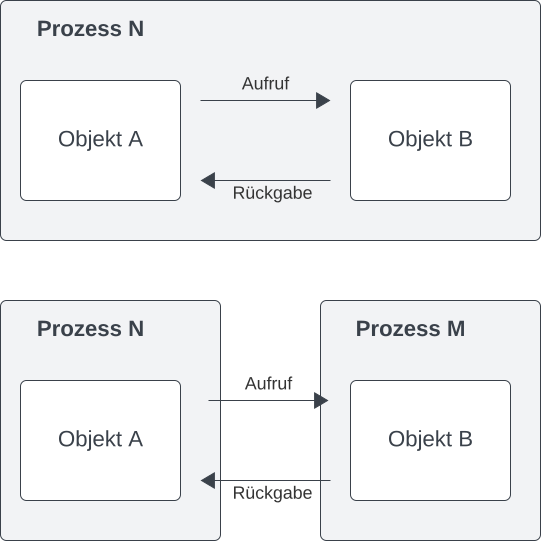
\includegraphics[scale=0.5]{chapters/fopt5/img/rmi/processcall}
    \caption{Zwei unterschiedliche Objekte in unterschidlichen Aufrufsituationen. Im oberen Beispiel befinden sich die Objekte im selben Adressraum, im unteren Beispiel in unterschiedlichen Adressräumen - diese Situation kommt bei der Nutzung von RMI vor (Quelle: in Anlehnung an \cite[311 f., Abbildung 6.1 und 6.2]{Oec22})}
    \label{fig:processcall}
\end{figure}

\noindent
Die \textbf{Vereilungstransparenz} wird bei \textbf{RMI} über \textbf{Stubs} und \textbf{Skeletons} realisiert.\\

\noindent
Ein \textbf{Stub} implementiert dieselbe Schnittstelle wie das Objekt, das über Fern-Methodenaufrufe \ul{auf dem Server gesteuert werden soll}.

\noindent
Ein \textbf{Skeleton} nimmt die Nachrichten, die vom \textbf{Stub} über die aufgebaute \textbf{TCP}-Verbindung gesendet werden, entgegen und ruft die Methoden auf dem entsprechenden Server-Objekt auf.\\
$\rightarrow$ Ein \textbf{Skeleton} besitzt die Struktur eines \textbf{TCP}-Servers.

\begin{figure}
    \centering
    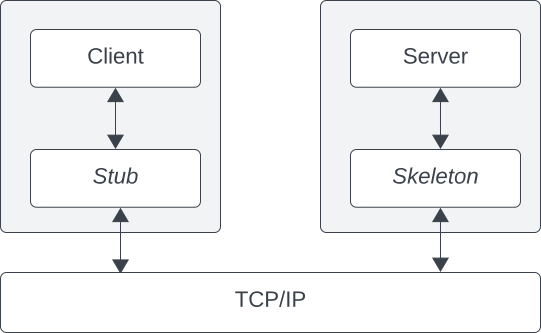
\includegraphics[scale=0.4]{chapters/fopt5/img/rmi/stubskeleton}
    \caption{Prinzip der Kommunikation zwischen RMI-Client und -Server. (Quelle: in Anlehnung an \cite[312, Bild 6.3]{Oec22})}
    \label{fig:stubskeleton}
\end{figure}

\begin{tcolorbox}
    Struktur einer RMI Anwendung\footnote{vgl. im folgenden \cite[162 ff.]{HM05}; \textbf{Stubs} und \textbf{Skeletons} werden in unserem Fall automatisch generiert.}:\\


    \noindent
    \textbf{RMI-Client}\\
    Ein \textbf{RMI-Client} fragt bei einem \textbf{RMI-Namensdienst} eine Referenz auf ein entferntes Objekt an, das danach wie ein lokales Objekt behandelt wird.
    Die notwendige Netzwerk-Kommunikation für diese Methodenaufrufe ist transparent und wird automatische abgewickelt.\\


    \noindent
    \textbf{Stub-Objekt}
    \begin{itemize}
        \item Ein \textbf{Stub-Objekt} ist ein \textbf{Stellvertreter} für das entfernte Objekt bei dem RMI-Server.
        Methodenaufrufe des \textbf{RMI-Clients} auf ein entferntes Objekt werden an das Stub-Objekt \textit{delegiert}.
        \item Verantwortlichkeiten: Weiterleitung von Methodenaufrufe an das entfernte Objekt. \textit{Marshalling} von Übergabeparametern und \textit{unmarshalling} von Rückgabewerten\footnote{
          Serialisierung: Umwandeln einer Objektstruktur in ein speicherbares Format. Marshalling bezieht sich auf das Bewegen von Objekten zwischen Threads und Programmen, wofür auch eine Form von Serialisierung notwendig ist. S. a. ``Marshalling (computer science): \url{https://en.wikipedia.org/wiki/Marshalling_(computer_science)} - abgerufen 1.2.2024
        }.
        \item Der Stub wird für jede Anwendung automatisch erzeugt (vgl.\cite[313]{Oec22}).
    \end{itemize}\\

    \noindent
    \textbf{Skeleton-Objekt}\\
   Ein \textbf{Skeleton-Objekt} ist ein \textit{server-seitiger} \textbf{Stellvertreter} für das aufrufende Objekt bei dem RMI-Server, uns unterstützt ebenfalls  \textit{Marshalling} von Übergabeparametern und \textit{unmarshalling} von Rückgabewerten. Das Sekeleton-Objekt ist als Programmteil in der RMI-Implementierung dabei und kann für alle RMI-Anwendungen verwendet werden (vgl.\cite[313]{Oec22}).\\

    \noindent
    \textbf{RMI-Registry}\\
    Die \textbf{RMI-Registry} realisiert einen \textit{Namensdienst}: Eine Abbildung von Namen auf entfernte Objekte.\footnote{
        s.a: ``Kapitel 6: Verteilte Objekte durch RMI``: \url{https://www.informatik.uni-marburg.de/~mathes/download/k6.pdf}, ``Distributed object communication``: \url{https://en.wikipedia.org/wiki/Distributed_object_communication} - beides abgerufen 1.2.2024
    }. \\
    Der \textbf{RMI-Client} fordert hier die Referenzen auf entfernte Objekte an.\\

    \noindent
    \textbf{RMI-Server}\\
    Ein \textbf{RMI-Server} instanziiert ein entferntes Objekt und registriert es unter einem Namen bei der \textbf{RMI-Registry}, und wartet \textit{passiv} auf den Aufruf einer Methode durch den \textbf{RMI-Client}.

\end{tcolorbox}

\begin{figure}
    \centering
    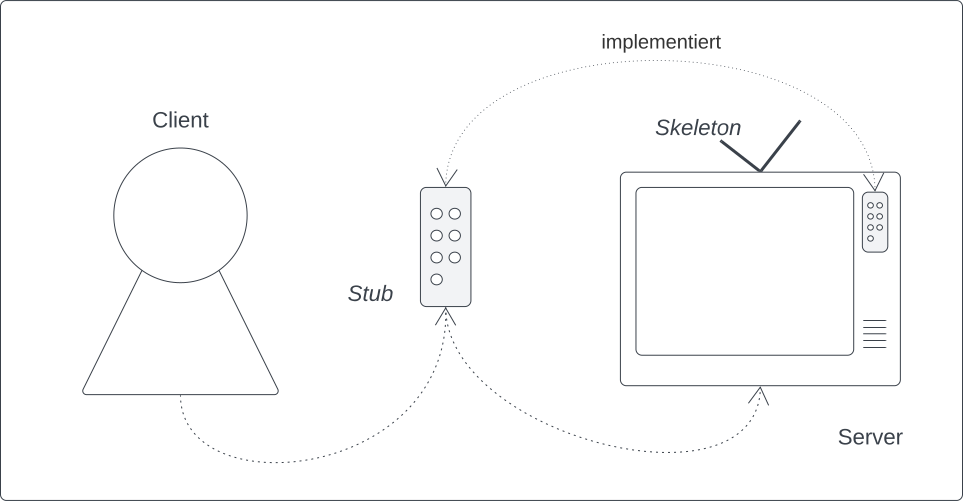
\includegraphics[scale=0.35]{chapters/fopt5/img/rmi/tv}
    \caption{Eine Illustration der im Lehrbuch verwendeten RMI-Metapher. Ein Client will ein entferntes Objekt (TV) bedienen. Hierzu verwendet er Methodenaufrufe, die vom Stub (Fernbedienung) weitergeleitet werden. Die Methoden werden vom Skeleton (Fensehantennen) an das Objekt auf dem Server (TV) weitergeleitet. (Quelle: eigene)}
    \label{fig:tv}
\end{figure}
